\section{Magnetization}\label{sec:res:magnet}
	\subsection{Observable}\label{sec:res:magnet:observable}
		\Observable{Metropolis}{Magnetization}{magnetization}
		\Observable{Wolff}{Magnetization}{magnetization}
		Studying the total absolute magnetization per spin for the Metropolis (\cref{fig:obs:Metropolis:Magnetization}) and Wolff (\cref{fig:obs:Wolff:Magnetization}) algorithms shows that, for low temperatures, the magnetization tends to $1$, indicating the existence of a quasi-ordered low-temperature state. With increasing temperature, the magnetization decreases steadily at first and then rapidly until it slowly levels out in the unordered high-temperature state. One can also see finite-size effects as, for increasing lattice sizes, the form of the curve becomes more pronounced. The errors can be found in~\Cref{sec:errors:magnetization} of~\Cref{chap:errors}.
		
		\paragraph{Magnetization Squared per Spin}\label{sec:res:magnetsquare} The plots for the absolute total magnetization per spin, its autocorrelation function, and integrated autocorrelation time can be found in~\Cref{sec:observables:magnetization_squared}, and the errors can be found in~\Cref{sec:errors:magnetizationsquare} of~\Cref{chap:errors}.
	
	\subsection{Magnetic Susceptibility}\label{sec:res:xs}
		\Observable{Metropolis}{MagneticSusceptibility}{magnetic susceptibility}
		\Observable{Wolff}{MagneticSusceptibility}{magnetic susceptibility}
		The magnetic susceptibility $\chi$ can be derived from $\langle M \rangle$ and $\langle M^2 \rangle$ according to~\Cref{eq:magnetic_suceptibility}.  Comparing the curve of the Metropolis (\cref{fig:obs:Metropolis:MagneticSusceptibility}) and Wolff (\cref{fig:obs:Wolff:MagneticSusceptibility}) algorithms reveals a similar form. The magnetic susceptibility is small for low and high temperatures. A peak exists near the critical temperature, which slowly shifts to the left and becomes narrower as the lattice size increases and the peak's magnitude decreases. The errors can be found in~\Cref{sec:errors:magneticsusceptibility} of~\Cref{chap:errors}.
		
		Near criticality, the curve of $X$ obtained using the Wolff algorithm is substantially smoother, which can be attributed to the reduced critical slowing down effects experienced by the Wolff algorithm.
	
	\subsection{Estimating \texorpdfstring{$T_C$}{T} using the Magnetic Susceptibility \texorpdfstring{$\chi$}{X}}\label{sec:res:temperature}
		As shown by~\citet[eq. 3]{shifted}, there exists a shifted temperature $T^*$ that asymptotically approaches the critical temperature $T_C$ for an infinite lattice
		\begin{equation}\label{eq:shifted_temperature}
			T^*(L) \approx T_C + \frac{\pi^2}{4c (\ln{L})^2}.
		\end{equation}
		The shifted temperature gives us a way to estimate the critical temperature $T_C$. To confirm the correlation between lattice size and shifted temperature, we now take the maximum magnetic susceptibility $\chi_\text{max}$ per lattice size from~\Cref{fig:obs:Metropolis:MagneticSusceptibility} and plot the temperature $T$ where it occurs against $(\ln{L})^{-2}$ in~\Cref{fig:critical_temperature}.
		\begin{figure}[htbp]
			\centering
			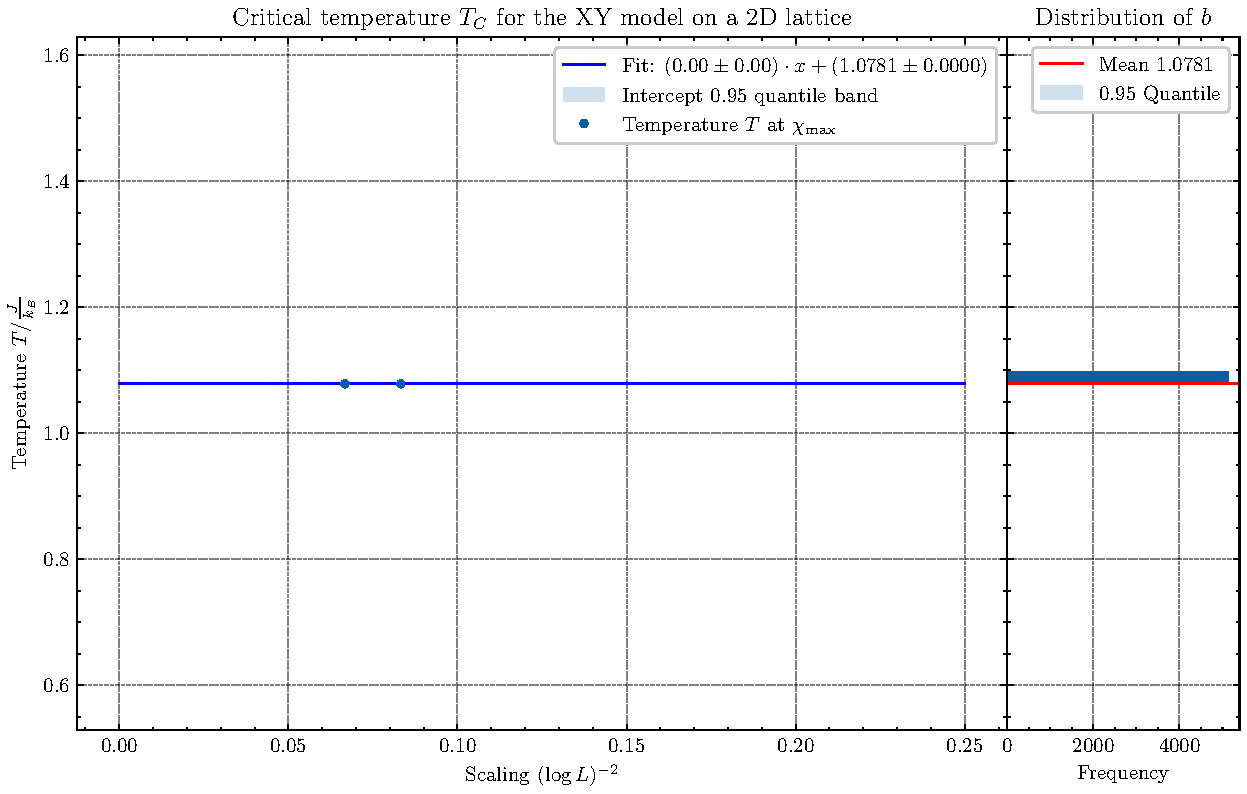
\includegraphics[width=0.8\textwidth]{../figures/Metropolis/Critical_Temperature.pdf}
			\caption[Estimating $T_C$ using the Metropolis algorithm by plotting $T$ where $\chi$ is maximal against $(\ln L)^{-2}$]{The temperature at which $\chi$ is maximal against $(\ln L)^{-2}$ yields a linear correlation and confirms~\Cref{eq:shifted_temperature} for the Metropolis algorithm.}
			\label{fig:critical_temperature}
		\end{figure}
		\begin{figure}[htbp]
			\centering
			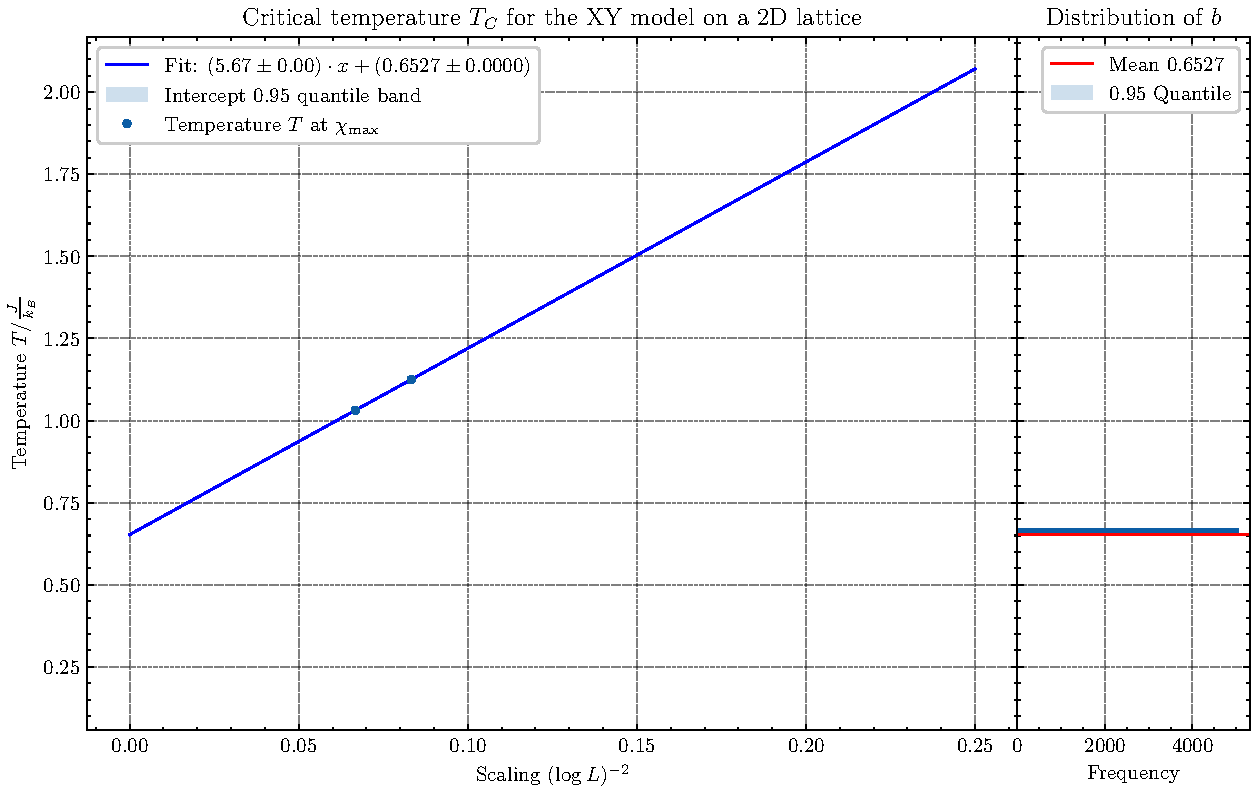
\includegraphics[width=0.8\textwidth]{../figures/Wolff/Critical_Temperature.pdf}
						\caption[Estimating $T_C$ using the Wolff algorithm by plotting $T$ where $\chi$ is maximal against $(\ln L)^{-2}$]{The temperature at which $\chi$ is maximal against $(\ln L)^{-2}$ yields a linear correlation and confirms~\Cref{eq:shifted_temperature} for the Wolff algorithm.}
			\label{fig:critical_temperature_wolf}
		\end{figure}
		
		We fitted a linear regression model using a least-squares method against our data points, which confirms the correlation of lattice size and shifted temperature. The intercept of the fit gives the estimate for the critical temperature. To estimate our errors, we used a bootstrap approach by resampling $\num{10 000}$ times from our measurements and redoing our linear regression model each time. As seen on the right side of~\Cref{fig:critical_temperature}, the distribution of intercepts $b$ follows a Gaussian distribution and therefore the central limit theorem. The standard deviation $\sigma$ of our bootstrapped intercepts was taken as the error of our estimate of the critical temperature
		\begin{equation}
			T_{C, \text{Metropolis}} = \SI{0.886(12)}{\J\per\kb}.
		\end{equation}
		Doing the same for the Wolff algorithm (\cref{fig:critical_temperature_wolf}) for our $\chi_\text{max}$ obtained from~\Cref{fig:obs:Wolff:MagneticSusceptibility} yields
		\begin{equation}
			T_{C, \text{Wolff}} = \SI{0.8978(14)}{\J\per\kb}.
		\end{equation}
		Comparing the two estimates shows that the Wolff algorithm yielded a more precise measurement. The increase in precision can be attributed to the reduced critical slowing-down effects experienced by the Wolff algorithm.
		
		We can compare our result with some literature values:
		\begin{itemize}
			\item In~\citet{literature_gpu}, the authors used a GPU-based Monte Carlo approach to estimate the critical temperature to $T_C=\SI{0.8935(1)}{\J\per\kb}$.
			\item In~\citet{literature_cpu}, the authors used a CPU-based Monte Carlo approach to estimate the critical temperature to $T_C=\SI{0.89213(10)}{\J\per\kb}$.
			\item A theoretical transfer matrix approach employed by~\cite{literature_theo} led to a critical temperature of $T_C \approx \SI{0.8916}{\J\per\kb}$.
		\end{itemize}
		These literature values are compatible with our estimated $T_{C, \text{Metropolis}}$ which indicates that our implementation is correct and our temperature \emph{zoom} procedure works. Our errors are bigger by a factor of $\sim 100$ than those of others, which is a result of our time and resource constraints. The errors of our estimate $T_{C, \text{Wolff}}$ are smaller by a factor of $\sim 10$ than those of the Metropolis algorithm, which is another indication of the superiority of the Wolff algorithm near the critical temperature. The estimate itself is numerically larger than expected, and the literature values are therefore outside of our errors. This is not surprising, as the literature values were, at least for those obtained using Monte Carlo methods, simulated on larger lattice sizes ($L = 512$) and used more mathematical insights when fitting $\chi$.

		When zooming in on the $\chi$ peak for the Metropolis (\cref{fig:critical_temperature_zoom}) and Wolff (\cref{fig:critical_temperature_wolf_zoom}) algorithms, we see further advantages of  using the Wolff algorithm. The data points follow a very predictable trajectory,  which gives us the confidence that if we were to increase the temperature scanning depth to $\geq 3$, we would not zoom in on the wrong neighbourhood.
		\begin{figure}[htbp]
			\centering
			\includegraphics[width=0.8\textwidth]{../figures/Metropolis/Critical_Temperature_Zoom.pdf}
			\caption[Estimating $T_C$ using the Metropolis algorithm by plotting $T$ where $\chi$ is maximal against $(\ln L)^{-2}$]{The temperature at which $\chi$ is maximal against $(\ln L)^{-2}$ yields a linear correlation and confirms~\Cref{eq:shifted_temperature} for the Metropolis algorithm.}
			\label{fig:critical_temperature_zoom}
		\end{figure}
		\begin{figure}[htbp]
			\centering
			\includegraphics[width=0.8\textwidth]{../figures/Wolff/Critical_Temperature_Zoom.pdf}
			\caption[Estimating $T_C$ using the Wolff algorithm by plotting $T$ where $\chi$ is maximal against $(\ln L)^{-2}$]{The temperature at which $\chi$ is maximal against $(\ln L)^{-2}$ yields a linear correlation and confirms~\Cref{eq:shifted_temperature} for the Wolff algorithm.}
			\label{fig:critical_temperature_wolf_zoom}
		\end{figure}
